\begin{figure}
\centering
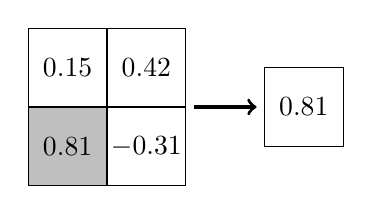
\begin{tikzpicture}

\fill[draw=black,color=lightgray] (0,0) rectangle (1,1);
\draw (0,0) rectangle (1,1) node[pos=0.5] {$0.81$};
\draw (0,1) rectangle (1,2) node[pos=0.5] {$0.15$};
\draw (1,0) rectangle (2,1) node[pos=0.5] {$-0.31$};
\draw (1,1) rectangle (2,2) node[pos=0.5] {$0.42$};

\draw (3,0.5) rectangle (4,1.5) node[pos=0.5] {$0.81$};
\draw [->,very thick] (2.1,1) -- (2.9,1) ;

\end{tikzpicture}

\caption{Example of a 2x2 max pool operation. In a 2x2 region, the largest value is chosen while the other values are ignored.}
\label{fig:maxpool}
\end{figure}
